\RequirePackage{ifpdf}
\documentclass[11pt, final]{ucthesis}
% Look at the README first!  It's short!

%%% \documentclass[11pt/12pt/10pt, final/draft/comment]{ucthesis}
%%% The first argument is the text size. The second argument changes
%%% The margins and the spacing.
%%% FINAL mode prints double spaced with figures and thesis margins.
%%% DRAFT mode prints single-spaced with 1" margins, with slightly
%%%   narrower margins for the figure captions so that they stand out.
%%% COMMENT mode prints an extra wide right margin and tiny margins
%%% everywhere else. This allows your committee plenty of room to add
%%% comments.
%%% Margins can be changed in the last lines of the ucthesis.cls
%%% with the geometry command.

% This information will get stored inside the PDF file
%\pdfinfo{
%       /Title      (U. C. Berkeley Dissertation)
%       /Author     (Your Name Here)
%       /Keywords   ()
%    }

% This gives you control over how far down in the hierarchy the
% table of contents will print. I use 2.
\setcounter{tocdepth}{2}

% This allows me to add directories to the graphics path
% so that I don't need to specify directories in the individual
% LATEX paths.
% EACH PATH MUST END IN A '/'
% In other words, \includegraphics{Fig1} will first look in the current
% directory, but if it can't find the file Fig1, it will  look for
% SUBDIRECTORY/Fig1 . If that's not there, it will look next in
% SUBDIRECTORY2/Fig1 . If it finds that, it will ignore anything after
% SUBDIRECTORY2.
%
% As I have them now, they are:
\graphicspath{{introduction_figs/},{MORE_figs/},{EVENMORE_figs/}}

% ========================================= Extra commands
% Degree Symbol
\newcommand\degrees{\ensuremath{^\circ}}
\newcommand{\tab}{\hspace{5mm}}
\newcommand{\blankpage}{\clearpage ~ \newpage}


% ========================================= DOCUMENT
\begin{document}

% Declarations for Front Matter

% TITLE
\title{BeaverDam: Video Annotation Tool for Computer Vision Training Labels}

% NAME
% Note that this must be exactly as it appears in University records.
\author{Anting Shen}

% PREVIOUS DEGREES
% Put each previous degree on its own line in the following format:
\prevdegrees{}

% DATE OF GRADUATION
% This text will appear on the title page
% Note that degrees are only granted in Fall and Spring at Berkeley.
\degreemonth{Fall} \degreeyear{2016} \degree{Master of Science}
% This text will appear on the abstract page.
% For Berkeley, it should be identical to the graduation month.
\defensemonth{Fall} \defenseyear{2016}

% COMMITTEE MEMBERS
% You can have up to 5 members listed separately.
%After that, you throw them all into the "other members" category.
\numberofmembers{2}
    \chair{Professor Kurt Keutzer}
    \othermemberA{Professor Only Somewhat Important Guy}
    %\othermemberB{Professor Susan B. Anthony}
    %\othermemberC{Professor Arthur C. Clarke}
    %\othermemberD{Professor Dee Light}
    %\othermembers{Professor Too Many\\ Professor Another One}

% DEPARTMENT/DEGREE PROGRAM
%Your Department. Make sure this is the department and/or program
% name that you are enrolled in...
\field{Engineering - Electrical Engineering and Computer Sciences}

% CAMPUS NAME
% Your UC Campus, e.g., "Berkeley"
% Note that if you are not at Berkeley, you may have to modify the
% ucthesis.cls to change the wording on the Title page.
\campus{Berkeley}


\begin{frontmatter}

% ===============================================
% MAKE THE TITLE PAGE
% ===============================================
\maketitle


% ===============================================
% APPROVAL SIGNATURE PAGE
% ===============================================
% \approvalpage

% ===============================================
% Copyright Page
%
% The copyright page is optional. However, the University
% thesis guide says that a blank page should be inserted
% if no copyright information is included.
% ===============================================
\copyrightpage
% or the blankpage
% \blankpage

% ===============================================
% ABSTRACT
%
%   The Abstract should be stored in a file called abstract.tex
%   "It is preferred that the abstract text be less than 350 words"
%   Also generates a signature line at the end of the abstract
% ===============================================

 \abstract
    We present our annotation tool for frame-by-frame video bounding box annotation.
The framework has been used in conjunction with Amazon Mechanical Turk as well as standalone, to annotate datasets for Berkeley Deep Drive and BMW.
To accomplish this, we built upon ideas from previous works in this area, and we present our improvements and optimizations upon their user interfaces.
We also introduce the idea of tuning such an annotation tool to reduce researcher's friction, which we argue is just as important as improving workers' workflow due to the high cost of researcher time.
We share our experiences with existing tools, and our ideas (and code) for how to make the experience better for researchers.
We hope our findings and contributions further reduce the cost of producing a labeled video dataset, and introduce ideas that will improve the quality of such software in the future.

    \abstractsignature  % This prints a signature line for the chair to sign.
\endabstract

\end{frontmatter}

% ===============================================
% OPTIONAL MATERIAL
% Everything after this is optional and can appear in any order
% you desire.
\begin{optionalFrontMatter}

% ===============================================
% Dedication Page
% The dedication is optional.
% ===============================================
% \begin{dedication}
%  %Prints the text of the file dedication.tex centered vertically on the page.
%     \vspace*{\fill}
%     If you want, you can have a dedication...
%     \vspace*{\fill}
% \end{dedication}

% ===============================================
% TABLE OF CONTENTS
% \addcontentsline{toc}{chapter}{Contents}        % Put the table of contents in the table of contents
\tableofcontents

% COMMENT OUT THIS LINE IF YOU WANT TITLE HEADERS
% THROUGHOUT YOUR DOCUMENT
\pagestyle{plain}

% Insert the List of Figures and List of Tables after the TOC
% Like everything in this section, these are both optional.
% \listoffigures
% \listoftables

\begin{acknowledgements}
\addcontentsline{toc}{chapter}{Acknowledgements}
% The Acknowledgements section should be stored in a file called acknowledgments.tex
    Thanks to Professor Keutzer and everyone in our group for the motivation and advice, Kosta for the great support, and Bichen Wu \& Byung Gon Song for sharing in the struggles.

I'd also like to acknowledge Allen Wang, Sean Zhu, and Gabriel Arreola for contributing code to this project, coming up with awesome logos, and puns.

Lastly, thanks to all the turkers who helped annotate videos, especially David Tarr, Connor Munsinger, Allen Chov, and Aljosa Cucak for their feedback.

\end{acknowledgements}

% \begin{vitae}
% %% The Vitae section should be stored in a file called vitae.tex
%     
\begin{vitaesection}{Education}
\item [1992] University of South Babylon

B.S., Geological and Environmental Sciences

\item [2001] Diploma Factory State College

M.S., Geology

\item [2004] University of California Berkeley

Ph.D., Geology
\end{vitaesection}


\begin{vitaesection}{Personal}
\item [Born] April 18, 1906, 
San Francisco, California
\end{vitaesection}

%\begin{vitaesection}{Biographical Sketch}
%\item [] 
This can either be a formal CV, or include a more narrative biographical sketch. This is where people who discover your thesis decades down the road will find out about who you were.

%\end{vitaesection}


% \end{vitae}

% BLANK PAGE AFTER VITAE
\blankpage

\end{optionalFrontMatter}
%%%% END FRONT MATTER...


% ============================= DISSERTATION TEXT
% Begins regular arabic numeral page numbers...

\begin{dissertationText}
\renewcommand{\baselinestretch}{1.66}

% CHAPTERS
\chapter{Introduction
    \label{chap:introduction}}    % Put the title of the first chapter on this line
    Deep learning applications in recent years have come to require rapidly growing amounts of labeled training data.
Often, accuracies can be boosted by adding data as much as by spending years on algorithmic development.
For example, on the VOC07 benchmark, Faster-RCNN~\cite{FasterRCNN} with VGG-16 was able to eliminate 27.5\% of errors in the much older R-CNN~\cite{RCNN} backed by an equally old neural network architecture (mAP improved from 58.5 to 69.9). 
However, simply by including additional data from VOC12 and COCO, 29.5\% of the remaining error was eliminated (mAP improved from 69.9 to 78.8). 

\begin{figure}[h]
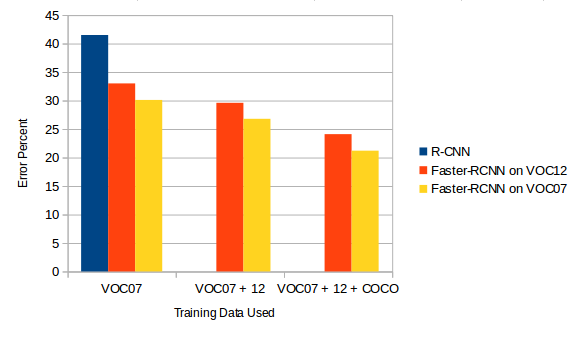
\includegraphics[width=14cm]{figs/data_vs_error.png}
\centering
\caption{Improvement of error as data increases, compared to error improvements due to algorithm improvements. 
As we can see by comparing the drop from RCNN to Faster-RCNN on VOC07 only, and the drop from adding training data to Faster-RCNN, increasing data contributes significantly to error reduction.}
\end{figure}

Therefore, for real-world application development, data can be cheaper and more effective than scientists. 
While many existing tools support image classification -- it is even built into Amazon Mechanical Turk (MTurk) -- and some tools support bounding box labeling in images, few tools exist for frame-by-frame labeling in videos. 
VATIC~\cite{Vatic} stands out as being one of the best, as not only does it make high quality annotations one of its main goals, but also cost and scalability. 

My work borrows and improves upon many concepts and results from VATIC's user studies, but I focus on an additional goal that is extremely important in creating datasets for real applications. That goal is researcher happiness.
Although VATIC extensively tested its ``User Interfaces'', I argue in chapter~\ref{chap:experimenter} that both the annotators and the experimenters are users, and the interfaces should be smooth for both when creating a tool.

Then, in chapter~\ref{chap:annotator}, I discuss my take on VATIC's User Interface principles for the annotator, and improvements upon them.

I also release all related code for BeaverDam, my video labeling platform, on Github.\footnote{http://github.com/antingshen/beaverdam}

\section*{Related Work}
\label{sec:related}

Static image annotators

Youtube video dataset

Vatic, LabelMe, etc

Things other people cite

KITTI, Berkeley group, samasource
  %% Adds the contents of the file introduction.tex
    %%% The file should have no preamble -- the chapter body.

\chapter{Interference
    \label{chap:circles}}  % Put the title of next chapter on this line
    Another great chapter!


Blah blah blah blah blah blah blah blah blah blah blah blah blah blah blah. Blah blah blah blah blah blah blah blah blah blah blah blah blah blah blah. Blah blah blah blah blah blah blah blah blah blah blah blah blah blah blah. Blah blah blah blah blah blah blah blah blah blah blah blah blah blah blah. Blah blah blah blah blah blah blah blah blah blah blah blah blah blah blah. Blah blah blah blah blah blah blah blah blah blah blah blah blah blah blah.  Blah blah blah blah blah blah blah blah blah blah blah blah blah blah blah. Blah blah blah blah blah blah blah blah.
\begin{figure}[h!]
\begin{center}
\caption{Blah blah blah blah blah blah blah blah blah blah blah blah blah blah blah. Blah blah blah blah blah blah blah blah blah blah blah blah blah blah blah. Blah blah blah blah blah blah blah blah blah blah blah blah blah blah blah.  Blah blah blah blah blah blah blah blah blah blah.}
\label{Figure1}
\end{center}
\end{figure}

Blah blah blah blah blah blah blah. Blah blah blah blah blah blah
blah blah blah blah blah blah blah blah blah. Blah blah blah blah
blah blah blah blah blah blah blah blah blah blah blah. Blah blah
blah blah blah blah blah blah blah blah blah blah blah (see Figure
\ref{Figure1}) blah blah. Blah blah blah blah blah blah blah blah
blah blah blah blah blah blah blah. Blah blah blah blah blah blah
blah blah blah blah blah blah blah blah blah. Blah blah blah blah
blah blah blah blah blah blah blah blah blah blah blah. Blah blah
blah blah blah blah blah blah blah blah blah blah blah blah blah.


say, ``Blah blah blah blah blah blah blah blah blah blah blah blah
blah blah blah."

And so it goes...
        %% Adds the contents of blahblah.tex here

\chapter{Conclusion
    \label{chap:conclusion}}
    We have presented numerous improvements to existing video annotation tools.
We first argued that optimizing for researcher time is as important, if not more important than optimizing for worker efficiency, and showed our contributions in that area.
Then we demonstrated several ideas that allow for easier annotation by the workers that we discovered in our experiments.
We showed how BeaverDam enables cheaper annotations to create large datasets that improve model accuracies in production.

As BeaverDam is designed to be extensible, we hope that the platform will adapt to new types of annotations.
BeaverDam's modular designs shine best when new types of data, such as point clouds from LIDAR, require human labeling in the future.





% Start Bibliography on its own page
\clearpage

% This was the most significant change I made to the original style file.
% The template now accepts the IEEE-style .bib files that I was already using
% for my papers.  -Niels Hoven 5/24/2005
% You can substitute the name of another bibliography style file here.
\bibliographystyle{IEEEtran}
\addcontentsline{toc}{chapter}{Bibliography}
\ssp    % SINGLE SPACE REFERENCES (optional)

\bibliography{IEEEfull,cog_radio}


% ------------------- OPTIONAL APPENDICES
\appendix
\chapter{Allocated spectrum for communications
    \label{appen:commspec}}
   
source: Comsearch~\cite{Comsearch}

\begin{table}[htp]
 \begin{center}\begin{tabular}[t]{|c|c|}
 \hline
Category &  Allocation \\
\hline

Microwave & 609 MHz  \\
\hline

Broadcast & 423 MHz\\
\hline

Satellite & 188 MHz  \\
\hline

Point-to-Multipoint & 203 MHz  \\
\hline

PCS/Cellular & 193 MHz   \\
\hline

ISM & 110 MHz    \\
\hline

Other & 1274 MHz   \\
\hline

\end{tabular}
\end{center}
  \caption{\footnotesize{Spectrum under 3 GHz}
   \label{table:categories}}
\end{table}

\end{dissertationText}
\end{document}

% Congratulations, Doc!
